\ifdefined \wholebook \else\documentclass[oneside]{book}\usepackage{EdlBook}\graphicspath{{figures/}}
\addto\captionsicelandic{\renewcommand{\chaptername}{Kafli}}
%\setsecnumdepth{chapter}
\begin{document}
%%%
%
\setcounter{chapter}{12} % one less than this chapter
%
%%%
\fi
%%%%%%%%%%%%%%%%%%%%%%%%%%%%%%%%
%      CHAPTER TEXT GOES BELOW
%%%%%%%%%%%%%%%%%%%%%%%%%%%%%%%%

\renewcommand{\thefigure}{\arabic{figure}}
\counterwithout{equation}{chapter}

\chapter{Varmafræði}

\section{Varmaorka}

Eins og allir hlutir hafa eðlismassa þá hafa allir hlutir eðlisvarma:

\begin{tcolorbox}
\begin{definition}
Lítum á einsleitan hlut með massa $m$. Þá er \textbf{varmaorkan}, $Q$, sem þarf til þess að hita hlutinn um hitastig $\Delta T$, gefin með:
\begin{align*}
    Q = cm\Delta T,
\end{align*}
þar sem $c$ er fasti sem kallast \textbf{eðlisvarmi} og er háður efnasamsetningu hlutarins.
\end{definition}
\end{tcolorbox}

\subsection{Bræðsluvarmi og gufunarvarmi}

Í þessu námskeiði munum við skoða eftirfarandi ástandsform: \textbf{fastform}, \textbf{vökvaform} og \textbf{gasform}. Tæknilega séð eru til fleiri ástandsform heldur en þessi þrjú. Sem dæmi um önnur ástandsform þá má nefna: \textbf{rafgas} (\emph{e.} \textbf{plasma}); \textbf{Bose-Einstein þéttivatn} (\emph{e.} \textbf{Bose-Einstein condensate}) og \textbf{ofurflæðiefni} (\emph{e.} \textbf{superfluid}).

\begin{tcolorbox}
\begin{definition}
Lítum á einsleitan hlut með massa $m$. Þá er:
\begin{enumerate}[label = \textbf{(\roman*)}]
    \item Varmaorkan, $Q_b$,  sem þarf til þess að bræða hlutinn, gefin með:
\begin{align*}
    Q_b = mL_b
\end{align*}
þar sem $L_b$ er fasti sem kallast \textbf{bræðsluvarmi} og er háður efnasamsetningu hlutarins.
    \item Varmaorkan, $Q_g$,  sem þarf til þess að sjóða hlutinn, gefin með:
\begin{align*}
    Q_g = mL_g
\end{align*}
þar sem $L_g$ er fasti sem kallast \textbf{gufunarvarmi} og er háður efnasamsetningu hlutarins.
\end{enumerate}

\end{definition}
\end{tcolorbox}

\begin{table}[H]
    \centering
    \vspace{-0.2cm}
    \begin{tabular}{|c|c|c|c|c|c|}
        \hline
        Efni & Eðlisvarmi & Bræðsluhitastig & Bræðsluvarmi & Gufunarhitastig & Gufunarvarmi\\ \hline \hline
        Vatn & \SI{4.19}{kJ/kg.K} & \SI{0}{\celsius} & \SI{333}{kJ/kg} & \SI{100}{\celsius} & \SI{2260}{kJ/kg} \\ \hline
        Ís & \SI{2.09}{kJ/kg.K} & \SI{0}{\celsius} & \SI{333}{kJ/kg} & \SI{100}{\celsius} & \SI{2260}{kJ/kg} \\ \hline
        Kvikasilfur & \SI{0.14}{kJ/kg.K} & \SI{-39}{\celsius} & \SI{11}{kJ/kg} & \SI{357}{\celsius} & \SI{296}{kJ/kg} \\ \hline
        Blý & \SI{0.128}{kJ/kg.K} & \SI{327}{\celsius} & \SI{25}{kJ/kg} & \SI{1750}{\celsius} & \SI{870}{kJ/kg} \\ \hline
        Járn & \SI{0.449}{kJ/kg.K} & \SI{1540}{\celsius} & \SI{289}{kJ/kg} & \SI{3020}{\celsius} & \SI{6340}{kJ/kg} \\ \hline
    \end{tabular}
    \caption{Eðlisvarmi, bræðsluvarmi og gufunarvarmi nokkurra efna.}
\label{tab}
\end{table}

\section{Kjörgas}

\begin{tcolorbox}
\begin{definition}
Lítum á gas (safn af sameindum). Við táknum með:
\begin{itemize}
    \item $N$: Heildarfjöldi sameinda í gasinu.
    \item $n$: Mólfjöldi sameinda í gasinu.
    \item $N_A$: Avogadrosartalan, $N_A = \SI{6.02e23}{1/mól}$, sem er þannig að $n = \frac{N}{N_A}$.
    \item $k_B$: Boltzmann-fastinn, $k_B = \SI{1.38e-23}{J/K}$.
    \item $R$: Gasfastinn, sem er skilgreindur þannig að $R = N_A k_B = \SI{8.315}{J/mól.K}$
    \item $M$: Heildarmassi sameindanna í gasinu.
    \item $m$: Frumeindamassi sameindanna, sem er þannig að: $M = Nm$.
    \item $u$: Frumeindamassinn, $u = \SI{1.66e-27}{kg}$.
    \item $\mu$: Mólmassinn, sem er skilgreindur þannig að $\mu = \frac{M}{n}$.
\end{itemize}
\end{definition}
\end{tcolorbox}

\begin{tcolorbox}
\begin{theorem}
Látum $Q$ tákna varmaorkuna sem þarf til þess að hita gas með eðlisvarma $c$ og heildarmassa $M$ (þar sem rúmmáli gassins er haldið föstu) um hitastig $\Delta T$. Þá gildir að:
\begin{align*}
    Q = cM\Delta T = Cn\Delta T
\end{align*}
Þar sem $n$ er mólfjöldinn í gasinu og $C$ er fasti sem nefnist \textbf{móleðlisvarmi}.
\end{theorem}
\end{tcolorbox}

\textbf{Útleiðsla:} Við höfum þá með smá umritun að:
\begin{align*}
    Q = cM\Delta T = cNm \Delta T = cn N_A m \Delta T = \left( \frac{c m}{k_B}R \right) n \Delta T = C_V n \Delta T.
\end{align*}
Þar sem við höfum skilgreint $C_V := \frac{cm}{k_B}R$. \qed

\vspace{0.2cm}

Það kemur síðan afar djúpstæð niðurstaða í varmafræði sem tengir móleðlisvarmann við \textbf{frelsisgráður} kerfisins. Þá kemur í ljós að rita megi $C = \frac{f}{2}R$, þar sem $f$ er fjöldi frelsisgráða sem sameindin hefur (nánar um nákvæma skilgreiningu á því síðar) og $R$ er gasfastinn. Sem dæmi má nefna að allar einatóma gassameindir (betur þekkt sem frumeindir, t.d. helíumssameindin $\text{He}$) hafa $f = 3$ frelsisgráður (eina fyrir hvern hraðaþátt sem frumeindin hefur) en allar tvíatóma sameindir (eins og súrefnissameindin $O_2$) hafa $f = \SI{5}{}$ frelsisgráður (ein fyrir hvern hraðaþátt massamiðjunnar og tveir fyrir hvernig er hægt að snúa sameindinni) en flest föst efni (t.d. járn, gull og blý) hafa $f = 6$ frelsisgráður (ein fyrir hvern hraðaþátt og þrjár fyrir hvernig er hægt að snúa sameindinni í kristalbyggingunni). Við höfum til dæmis að:

\begin{align*}
    \text{Vetnissameind, $\text{He}$:}& \hspace{1cm} C = \frac{c_{\text{He}}m_{\text{He}}}{k_B} R = \frac{3120 \cdot \SI{4,00}{} \cdot \SI{1.66e-27}{}}{\SI{1.38e-23}{}} R = \SI{2.497}{}R \approx \frac{3}{2}R. \\
    \text{Súrefnissameind, $O_2$:}& \hspace{1cm} C = \frac{c_{\text{$O_2$}}m_{\text{$O_2$}}}{k_B} R = \frac{656 \cdot \SI{32}{} \cdot \SI{1.66e-27}{}}{\SI{1.38e-23}{}} R = \SI{3.534}{}R \approx \frac{5}{2}R. \\
    \text{Gullsameind, $\text{Au}$:}& \hspace{1cm} C = \frac{c_{\text{Au}}m_{\text{Au}}}{k_B} R = \frac{129 \cdot \SI{197}{} \cdot \SI{1.66e-27}{}}{\SI{1.38e-23}{}} R = \SI{3.05}{}R \approx \frac{6}{2}R = 3R.
\end{align*}

\begin{tcolorbox}
\begin{definition}
Gas er sagt vera \textbf{kjörgas} ef það nýtur eftirfraandi skilyrða:
\begin{enumerate}[label = \textbf{(\roman*)}]
    \item Stærð sameindanna er hlutfallslega miklu minni heldur en meðalfjarlægðin á milli sameindanna. En það þýðir að við getum hunsað áhrif millisameindakrafta (eins og t.d.~rafsegulkrafturinn og þyngdarlögmálskrafturinn en ekki t.d.~eins og þverkraftarnir í árekstrunum).
    
    \item Allir árekstrar sameindanna við hvor aðra og ílátið sem þær eru innihaldnar í eru alfjaðrandi en það þýðir að orkan varðveitist í árekstrunum og að engin orka tapast út úr kerfinu heldur getur hún aðeins flust til á milli sameindanna við árekstrana.
\end{enumerate}
\end{definition}
\end{tcolorbox}

\begin{tcolorbox}
\begin{definition}
Lítum á gas þar sem að sameindir gassins hafa massa $m$ og meðalhraða $v$. Við skilgreinum meðalhitastig gassins þannig að það uppfylli eftirfarandi jöfnu:
\begin{align*}
  \frac{3}{2}k_B T = \frac{1}{2}mv^2 = K_{\text{hreyfi}}
\end{align*}
Þar sem $k_B = \SI{1.38e-23}{J/K}$ er fasti sem nefnist Boltzmann-fastinn.
\end{definition}
\end{tcolorbox}

Við sjáum hinsvegar að heildarorka sameindanna er $E = \frac{f}{2}k_B T$ því hverri frelsisgráðu fylgir orka sem jafngildir $\frac{1}{2}k_B T$. Vopnuð þessu þá erum við tilbúin til þess að leiða út gaslögmálið:


\begin{tcolorbox}
\begin{theorem}
\textbf{(Gaslögmálið)} Lítum á kjörgas sem samanstendur af $N$ sameindum með meðalhraða, $v$, inni í kassa sem hefur hliðarlengdir $\ell$. Þá er þrýstingurinn sem að sameindirnar verka með á kassann gefinn með:
\begin{align*}
    PV = N k_B T = nR T,
\end{align*}
þar sem $V = \ell^3$ er rúmmál kassans, $k_B = \SI{1.38e-23}{J/K}$ er fasti sem nefnist Boltzmann-fastinn, $T$ er meðalhitastig sameindanna, $n = \frac{N}{N_A}$ er mólfjöldi sameindanna þar sem $N_A = \SI{6.022e23}{1/mól}$ er Avagadrosartalan í kassanum og $R = k_B N_A = \SI{8.315}{J/mól.K}$ er gasfastinn.
\end{theorem}
\end{tcolorbox}

\textbf{Útleiðsla:} Hugsum okkur kassa með hliðarlengdir $\ell$ og rúmmmál $V = \ell^3$. Látum $N$ agnir með meðalhraða $v$ vera í kassanum. Við viljum vita hvaða þrýstingur er inni í kassanum. Rifjum því upp að:
\begin{align*}
    P = \frac{F_{\perp}}{A}
\end{align*}
og nýtum okkur að $F = \frac{\Delta p}{\Delta t}$. Látum því $\Delta t$ vera lítið tímabil. Við viljum finna skriðþungabreytingu veggjarins á tímanum $\Delta t$. Aðeins hlutfall agnanna mun berast að kassanum til þess að lenda í árekstrinum. Athugum fyrst að hraði agnanna er $\Vec{v} = (v_x, v_y, v_z)$ en að meðaltali mun hver hraðaþáttur vera jafn líklegur svo $v^2 = v_x^2 + v_y^2 + v_z^2 = 3v_x^2$ sem gefur þá að $v_x^2 = \frac{1}{3}v^2$. Fyrir lítil tímabil $\Delta t$ þá getum við gert ráð fyrir því að agnirnar nái aðeins að lenda í einum árekstri við hliðarlengdir kassans. Þá höfum við að heildarfjöldi agna sem lendir í árekstrinum er gefinn með:
\begin{align*}
    N \cdot \frac{v_x \Delta t}{2 \ell}
\end{align*}
Þar sem aðeins helmingur þeirra sameinda sem eru í fjarlægðinni $v_x \Delta t$ frá veggnum ná að lenda í árekstri við hann. Við athugum síðan að skriðþungabreytingin við það að sameindin lendi í árekstri við vegginn er gefin með $\Delta p_x = mv_x - (-mv_x) = 2mv_x$ því sameindin snýr við í árekstrinum og áreksturinn er alfjaðrandi svo hún skoppar til baka með sama hraða og hún lenti á veggnum með. En þar með höfum við að:
\begin{align*}
   P = \frac{F}{A} = \frac{\Delta p}{A\Delta t} = \frac{ \left( N \frac{v_x \Delta t}{2\ell} \cdot 2mv_x  \right)}{A\Delta t} = \frac{2N}{\ell A} \cdot \frac{1}{2}mv_x^2 = \frac{2N}{3A\ell}\frac{1}{2}mv^2 = \frac{N k_B T}{V}
\end{align*}
Þar sem við höfum notað skilgreininguna á hitastigi og að rúmmál kassans er $V = A \ell = \ell^3$. En þar með höfum við sýnt að: $PV = Nk_B T$. Það er síðan einfalt að umrita niðurstöðuna í samræmi við mólfjöldan með því að skilgreina $R := N_A k_B$. Þá má rita $PV = nRT$. \qed

\section{Fyrsta lögmál varmafræðinnar}

Hingað til í þessum kafla þá hefur mestmegnið af því sem við höfum gert verið vitleysa. Því við höfum allann tímann gert ráð fyrir því að engin vinna sé unnin á kerfinu sem að við erum að skoða. Það kemur reyndar í ljós að $Q = cm\Delta T$ er aðeins satt ef að engin vinna er unnin á kerfinu. Eða réttara sagt ef að efnið sem við erum að breyta hitastiginu á verður ekki fyrir neinni varmaþennslu eða við erum að breyta rúmmáli þess með einhverjum hætti. Til þess að laga þetta þá þurfum við að skipta yfir í alvöru útgáfuna af varmaorkunni og við þurfum að setja fram fyrsta lögmál varmafræðinnar.
\begin{tcolorbox}
\begin{theorem}
\textbf{(Fyrsta lögmál varmafræðinnar)} Látum $\Delta E$ tákna heildarorkubreytingu kerfis. Látum $W$ tákna heildarvinnuna sem er unnin af kerfinu og látum $Q$ tákna heildarvarmaorkubreytingu kerfisins. Þá gildir að:
\begin{align*}
    C n \Delta T = \Delta E = Q - W.
\end{align*}
Þar sem $C = \frac{f}{2}R$ er fasti sem nefnist móleðlisvarmi og $f$ táknar frelsisgráður sameindanna í kerfinu.
\end{theorem}
\end{tcolorbox}

Sér í lagi sjáum við þá að $Q = cm\Delta T$ gildir aðeins ef $W = 0$. Skoðum vinnuna sem er unnin á einhverju gasi við það að þjappa því inn um örlitla vegalengd $dx$. Við höfum þá að sú örlitla vinna, $dW$, er gefin með:
\begin{align*}
    dW = F_{\text{gas}} dx = P_{\text{gas}}A dx = P_{\text{gas}} dV
\end{align*}
En þar með sjáum við að til þess að ákvarða heildarvinnu þrýstingsins þá höfum við nefnilega:
\begin{align*}
    W = \int_{V_1}^{V_2} PdV
\end{align*}
En þetta er jafngilt því að finna flatarmálið undir ferlinum á $PV$-línuriti. En það er einfaldlega graf af þrýstingi gassins $P$ sem fall af rúmmáli hans, $V$. Ef við þekkjum þrýstinginn og rúmmálið og hitastigið í einum punkti í ferlinu þá er auðvelt að reikna hitastigið í öllum hinum punktunum. En ef við þekkjum hitastigið í öllum punktunum þá er auðvelt að álykta hver heildarorkubreyting gassins var, nefnilega $\Delta E = \frac{3}{2}k_B\Delta T$. Þar með er auðvelt að reikna hver varmaorkubreytingin var í gasinu, $Q = \Delta E + W$.


\section{Varmaferli}



\begin{tcolorbox}
\begin{definition}
Við segjum að varmaferli kjörgass sé:
\begin{enumerate}[label =\textbf{ (\roman*)}]
    \item \textbf{Jafnþrýstingsferli:} Ef þrýstingurinn, $P = \text{fasti}$.
    \item \textbf{Jafnrúmmálsferli:} Ef rúmmálið, $V = \text{fasti}$.
    \item \textbf{Jafnhitaferli:} Ef hitastigið, $T = \text{fasti}$.
    \item \textbf{Óvermið:} Ef varmabreytingin er $Q = 0$.
\end{enumerate}
\end{definition}

\begin{figure}[H]
    \centering
    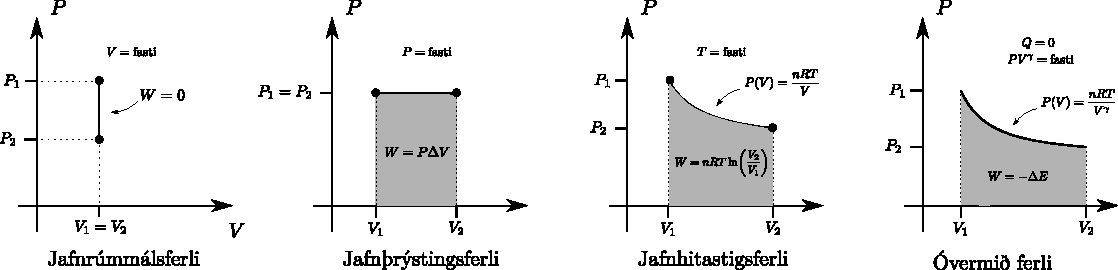
\includegraphics[width = \textwidth]{figures/varmaferlin.pdf}
\end{figure}
\end{tcolorbox}


\begin{tcolorbox}
\begin{theorem} Fyrir
\begin{enumerate}[label =\textbf{ (\roman*)}]
    \item Jafnþrýstingsferli gildir að $W$ og $\Delta E = Q$.
    \item Jafnrúmmálsferli gildir að $W = P \Delta V$ og $W = \Delta E + W = \gamma \Delta E$ þar sem $\gamma = \frac{f+2}{f}$ er óvermnisstuðullinn.
    \item Fyrir jafnhitaferli gildir að $\Delta E = 0$ og $W = Q = nRT\ln(\frac{V_2}{V_1})$.
    \item Óvermin ferli gildir að $Q = 0$ og $\Delta E = -W$.
\end{enumerate}
\end{theorem}
\end{tcolorbox}

\textbf{Útleiðsla:} \begin{enumerate}[label = \textbf{(\alph*)}]
    \item Við höfum þá að rúmmálsbreytingin er engin en þar með er $W = \int_{V_1}^{V_2} P dV = \SI{0}{J}$. Þar sem $V$ helst fast þá athugum við að:
    \begin{align*}
        \frac{P_1}{T_1} = \frac{P_2}{T_2}
    \end{align*}
    En þar með höfum við að heildarorkubreytingin er gefin með:
    \begin{align*}
        \Delta E = Cn \Delta T = Cn \left(T_2 - T_1 \right) = C n \left( \frac{P_2}{P_1} - 1\right) T_1 = Q - W = Q
    \end{align*}
    Svo við ályktum að:
    \begin{align*}
        \Delta E = C n \left( \frac{P_2}{P_1} - 1 \right)nT_1, \hspace{1cm} W = \SI{0}{J}, \hspace{1cm} Q = C n \left( \frac{P_2}{P_1} - 1 \right)nT_1.
    \end{align*}
    
    \item Ef þrýstingurinn helst fastur þá er $W = \int_{V_1}^{V_2}PdV = P \Delta V$. En þá er:
    \begin{align*}
        \frac{V_1}{T_1} = \frac{V_2}{T_2} \implies \Delta E = Cn \Delta T = Cn \left( \frac{V_2}{V_1}-1 \right)T_1 = \frac{f}{2} P \Delta V
    \end{align*}
    og þar með er heildarvarmabreytingin:
    \begin{align*}
        Q = \Delta E + W = \frac{f}{2} P \Delta V + P\Delta V = \left(\frac{f}{2}+1\right) P \Delta V = \gamma C P\Delta V
    \end{align*}
    Þar sem $\gamma := \frac{f+2}{f}$ er fasti sem nefnist óvermnisstuðullinn.
    
    \item Ef ferlið er jafnhitaferli þá er $\Delta E = 0$ og þar með er $Q = W$ og því nægir okkur að reikna vinnuna. En hún er gefin með:
    \begin{align*}
        W = \int_{V_1}^{V_2} PdV = \int_{V_1}^{V_2} \frac{nRT}{V}dV = \Bigg[ nRT \ln(V) \Bigg]_{V_1}^{V_2} = nRT \ln(\frac{V_2}{V_1}).
    \end{align*}
    \item Fyrir óvermin ferli gildir að stærðin $PV^\gamma$ er varðveitt stærð þar sem $\gamma = \frac{f+2}{f}$ er óvermnistuðullinn. Þar sem $Q = \SI{0}{J}$ þá er $\Delta E = -W$ og við athugum að hitastigsbreytingin er gefin með:
    \begin{align*}
        \frac{P_1 V_1}{T_1} = \frac{P_2 V_2}{T_2} \implies T_2 = \frac{P_2 V_2}{P_1 V_1}T_1
    \end{align*}
    En þar með er:
    \begin{align*}
        \Delta E = Cn\Delta T = Cn \left( \frac{P_2 V_2}{P_1 V_1} - 1 \right)T_1.
    \end{align*}
\end{enumerate}
\qed


\begin{tcolorbox}
\begin{theorem}
Gerum ráð fyrir að við höfum óvermið ferli. Þá er stærðin $PV^\gamma$ varðveitt eða með öðrum orðum þá er:
\begin{align*}
    P_1V_1^\gamma = P_2 V_2^\gamma
\end{align*}
Þar sem $\gamma$ er óvermnistuðullinn.
\end{theorem}
\end{tcolorbox}


\textbf{Útleiðsla:} Þar sem að vermisbreytingin er engin þá höfum við að:
\begin{align*}
    dE = -dW = -PdV = -\frac{nRT}{V}dV
\end{align*}
En við höfum líka að $dE = C_Vn dT$ svo við ályktum að:
\begin{align*}
    C_V n dT = - \frac{nRT}{V}dV \implies \frac{dT}{T} = - \frac{R}{C_V} \frac{dV}{V} = - \frac{R}{\frac{f}{2}R}\frac{dV}{V} = - \frac{2}{f} \frac{dV}{V}
\end{align*}
En við höfum þá með því að tegra að:
\begin{align*}
    \int_{T_1}^{T_2} \frac{dT}{T} = - \frac{2}{f}\int_{V_1}^{V_2} \frac{dV}{V}
\end{align*}
En stofnfallið af $\frac{1}{x}$ er $\ln(x)$ svo við fáum:
\begin{align*}
    \Big[ \ln(T) \Big]_{T_1}^{T_2} = - \frac{2}{f} \Big[ \ln(V) \Big]_{V_1}^{V_2} \implies \ln(T_2)-\ln(T_1) = -\frac{2}{f}\left( \ln(V_2) - \ln(V_1) \right)
\end{align*}
Sem gefur þar með að:
\begin{align*}
    \ln(T_1 V_1^{\frac{2}{f}}) = \ln(T_2 V_2^{\frac{2}{f}}) \implies T_1 V_1^{\frac{2}{f}} = T_2 V_2^{\frac{2}{f}}.
\end{align*}
En þar með ályktum við að stærðin $TV^{\frac{2}{f}}$ er varðveitt. Við getum umritað niðurstöðuna aðeins með því að taka eftir að $\frac{2}{f} = \gamma - 1$ svo $TV^{\gamma -1}$ er varðveitt stærð. En með því að nota gaslögmálið þá höfum við að $PV = nRT$ sem gefur að $T = \frac{PV}{nR}$ sem gefur þá sér í lagi að:
\begin{align*}
    TV^{\gamma -1} = \frac{PV}{nR}V^{\gamma -1} = \frac{1}{nR} PV^{\gamma}
\end{align*}
En þar með er ljóst að $PV^\gamma$ er varðveitt stærð. \qed

\newpage

\section{Dæmi}

\subsection*{Varmaorka}

\begin{tcolorbox}
Lítum á hlut með massa $m$. Varmaorkan, $Q$, sem þarf til þess að hita hlutinn um hitastig $\Delta T$, er gefin með $Q = cm\Delta T$ þar sem $c$ er fasti sem kallast eðlisvarmi og er háður efnasamsetningu hlutarins. Varmaorkan sem þarf til þess að bræða hlutinn er gefin með: $Q_{\text{b}} = mL_\text{b}$ þar sem $L_{\text{b}}$ er fasti sem kallast bræðsluvarmi. Varmaorkan sem þarf til þess að sjóða hlutinn er gefin með $Q_{\text{g}} = m L_{\text{g}}$ þar sem $L_{\text{g}}$ er fasti sem nefnist gufunarvarmi.
\begin{table}[H]
    \centering
    \vspace{-0.2cm}
    \begin{tabular}{|c|c|c|c|c|c|}
        \hline
        Efni & Eðlisvarmi & Bræðsluhitastig & Bræðsluvarmi & Gufunarhitastig & Gufunarvarmi\\ \hline \hline
        Vatn & \SI{4.19}{kJ/kg.K} & \SI{0}{\celsius} & \SI{333}{kJ/kg} & \SI{100}{\celsius} & \SI{2260}{kJ/kg} \\ \hline
        Ís & \SI{2.09}{kJ/kg.K} & \SI{0}{\celsius} & \SI{333}{kJ/kg} & \SI{100}{\celsius} & \SI{2260}{kJ/kg} \\ \hline
        Kvikasilfur & \SI{0.14}{kJ/kg.K} & \SI{-39}{\celsius} & \SI{11}{kJ/kg} & \SI{357}{\celsius} & \SI{296}{kJ/kg} \\ \hline
        Blý & \SI{0.128}{kJ/kg.K} & \SI{327}{\celsius} & \SI{25}{kJ/kg} & \SI{1750}{\celsius} & \SI{870}{kJ/kg} \\ \hline
        Járn & \SI{0.449}{kJ/kg.K} & \SI{1540}{\celsius} & \SI{289}{kJ/kg} & \SI{3020}{\celsius} & \SI{6340}{kJ/kg} \\ \hline
    \end{tabular}
\end{table}
\end{tcolorbox}

\begin{enumerate}[label = \textbf{Dæmi \thechapter.\arabic*.}]


\item \textit{(RK 19.12.)} Hversu mikla varmaorku þarf til að hita \SI{150}{g} af járni frá \SI{-20}{\celsius} í \SI{180}{\celsius}?


\item \textit{(RK 19.15.)} Hversu mikla varmaorku þarf til að sjóða \SI{16}{g} af kvikasilfri sem eru upphaflega við $\SI{22}{\celsius}$?

\item \textit{(RK 19.19.)} Tveir bílar (með massa $m = \SI{1000}{kg}$) lenda í árekstri. Báðir bílarnir voru á $\SI{80}{km/klst}$ hraða (í gagnstæða stefnu). Gerum ráð fyrir að öll orkan í árekstrinum losni í varmaorku sem fer í að hita bílana. Metið hversu mikið hitastig bílanna eykst ef báðir bílarnir eru úr járni.

\item \textit{(RK 19.21.)} Bráðin blýbyssukúla með massa \SI{30}{g} er tekin út úr ofni við $\SI{327}{\celsius}$ og sleppt ofan í einangrað ílát með \SI{100}{mL} af vatni við $\SI{20}{\celsius}$. Hvert verður lokahitstig kerfisins þegar það nær varmajafnvægi?

\begin{comment}
\item Þú ert með hálfan lítra af volgu kóki við stofuhita ($\SI{20}{\celsius}$). Til þess að kæla kókið þá bætiru $\SI{100}{g}$ af klaka út í kókið (\SI{-20}{\celsius}). Bráðnar allur ísinn? Ef svo, hvert er þá lokahitastigið? Ef ekki, hversu stór hluti af ísnum bráðnar? Gerið ráð fyrir að kókið hafi um það bil sama eðlisvarma og eðlismassa og vatn og að við erum með kókið í vel einangruðu ferðamáli.
\end{comment}

\item Krókódíll sem er \SI{2.9}{m} langur, \SI{60}{cm} breiður og \SI{350}{kg} þungur liggur í sólbaði. Ef styrkleiki sólarljóssins sem skín á bakið á honum er $\SI{500}{W/m^2}$ og hitastig hans er upphaflega $\SI{23}{\celsius}$, hversu langan tíma tekur það þá fyrir krókódílinn að ná $\SI{30}{\celsius}$? Eðlisvarmi líkamsvefja krókódílsins er að meðaltali $\SI{3400}{\joule\per\kilogram\per\kelvin}$.

\item \textbf{(Vorpróf 2019)} Viserion, dreki Daenerys Targaryen, ætlar að bræða niður hluta ísveggsins. Ísveggurinn er \SI{213}{m} hár og $\SI{91}{m}$ á þykkt. Til þess að færa her í gegnum vegginn þarf að bræða hringlaga gat sem hefur geisla $\SI{5.0}{m}$.
\begin{enumerate*}[label = \textbf{(\alph*)}]
    \item Hversu mikinn massa af ís þarf Viserion að bræða?
    
    \item Hitastig ísveggsins er iðuleg um $\SI{-17}{\celsius}$. Hversu mikla orku þarf til þess að bræða gat í vegginn af þessari stærð?
\end{enumerate*}

\item Englendingurinn Engilbert er mikill teunnandi. Honum finnst mjög mikilvægt að teið hans sé við nákvæmlega $\SI{67}{\celsius}$ þegar hann drekkur það.
\begin{enumerate*}[label = \textbf{(\alph*)}]
    \item Hann setur \SI{0.50}{L} af vatni við $\SI{7.0}{\celsius}$ í $\SI{2000}{W}$ hraðsuðuketil. Hversu lengi er hann að hita vatnið að suðu? (Gera má ráð fyrir að allur varminn fari í það að hita vatnið).
    
    \item Engilbert hellir sjóðandi heitu vatninu í tekönnu úr áli sem hefur massa $\SI{1.2}{kg}$ og eðlisvarma $\SI{900}{J/kg.K}$. Kannan er til að byrja með við stofuhita, $\SI{20}{\celsius}$. Hvert verður lokahitastig vatnsins í könnunni? (Gera má ráð fyrir því að enginn varmi tapist út í andrúmsloftið).
    
    \item Hversu miklum ís við $\SI{0}{\celsius}$ þarf Engilbert að bæta út í svo að lokahitastigið verði $\SI{67}{\celsius}$?
\end{enumerate*}

\end{enumerate}

\subsection*{Svör}

\begin{enumerate*}[label = \vspace{0.15cm} \textbf{(\arabic*)}]
  \item $Q = \SI{13,5}{kJ}$.
  \item $Q = \SI{5,5}{kJ}$.
  \item $\Delta T = \SI{0.55}{\celsius}$.
  \item $T = \SI{24,6}{\celsius}$.
  \item $\Delta t = \SI{2}{klst}$  $\SI{39}{mín}$ og $\SI{35}{s}$.
  \item $m_{\text{ís}} = \SI{6580}{tonn}$, $Q = \SI{2.4}{TJ}$.
  \item $\Delta t = \SI{97}{s}$, $T = \SI{72.8}{\celsius}$, $m_{\text{ís}} = \SI{30}{g}$.
\end{enumerate*}


\newpage

\subsection*{Gaslögmálið}

\begin{tcolorbox}
Gaslögmálið tengir saman þrýsting í kjörgasi, $P$, rúmmál þess, $V$ og hitastig þess, $T$ samkvæmt:
\begin{align*}
    PV = Nk_B T = nR T
\end{align*}

\vspace{-0.25cm}

Þar sem $k_B = \SI{1.38e-23}{J/K}$ er fasti sem nefnist Boltzmann-fastinn,
$N$ er heildarfjöldi sameindanna,
$n = \frac{N}{N_A}$ er mólfjöldi sameindanna, $N_A = \SI{6.022e23}{1/\text{mól}}$
er Avagadrosartalan og $R = k_B N_A = \SI{8.315}{J/\text{mól}.K}$ er gasfastinn.
\end{tcolorbox}

\begin{enumerate}[label = \textbf{Dæmi \thechapter.\arabic*.}]

\setcounter{enumi}{7}

\item \textit{(RK 18.20.)} Í $\SI{2.0}{L}$ íláti er búið að koma fyrir $\SI{3.0}{mólum}$ af gasi við hitastig $\SI{-120}{\celsius}$. Hver er þrýstingurinn í gasinu?

\item \textit{(RK 18.21.)} Í íláti nokkru er búið að koma fyrir $\SI{2.0}{mólum}$ af gasi við þrýsting $\SI{1.0}{atm}$ og hitastig $\SI{30}{\celsius}$. \begin{enumerate*}[label = \textbf{(\alph*)}]
    \item Hvert er rúmmál ílátsins?
    \item Ílátið er með fasta veggi og getur því ekki breytt rúmmáli sínu (slík ferli kallast jafnrúmmálsferli) Nú aukum við hitastigið á gasinu upp í \SI{130}{\celsius}. Hver er þrýstingurinn?
\end{enumerate*}


\begin{minipage}{\linewidth}

\begin{wrapfigure}{r}{1in}
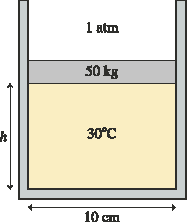
\includegraphics[width = 1in]{figures/dia-bulla.pdf}
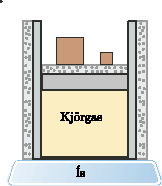
\includegraphics[width = 1in]{figures/kjorgas-bulla.pdf}
\end{wrapfigure}

\item \textit{(RK 18.24.)} Sívalningur með þvermál $þ = \SI{20}{cm}$ og hæð $h = \SI{40}{cm}$ inniheldur $\SI{50}{g}$ af súrefni ($O_2$) við $\SI{20}{\celsius}$. \begin{enumerate*}[label = \textbf{(\alph*)}]
    \item Hversu mörg mól af súrefni eru í sívalningnum?
    \item Hversu margar súrefnissameindir eru í sívalningnum?
    \item Hver er þrýstingurinn í gasinu?
    \item Hver er meðalhraði súrefnissameindanna?
\end{enumerate*}

\item \textit{(RK 18.58.)} Sívalingslaga bullan á myndinni hér til hægri hefur þvermál $þ = \SI{10}{cm}$ og bullulok með massa $m_b = \SI{50}{kg}$ sem hvílir ofan á $\SI{0.12}{mólum}$ af gasi sem eru til að byrja með við \SI{30}{\celsius} í jafnvægisstöðu kerfisins. Hver er hæðin $h$ í jafnvægisstöðunni?

\item \textit{(RK 19.10.)} Lítum á myndina hér til hægri. Tveir kassar með massa $m = \SI{2.0}{kg}$ og $M = \SI{5.0}{kg}$ sitja ofan á bulluloki með flatarmál $\SI{12}{cm^2}$ sem hefur massa $m_b = \SI{1.5}{kg}$. Inni í bullunni er $\SI{1.0}{mól}$ af einatóma kjörgasi við hitastig $ \SI{10}{\celsius}$. Nú setjum við risastóran klaka undir bulluna sem kælir gasið niður í \SI{0}{\celsius} við fastann þrýsting. \begin{enumerate*}[label = \textbf{(\alph*)}]
\item Hversu mikil verður rúmmálsbreyting gasins?
\item Hversu mikla vinnu vann gasið á bullunni við þetta ferli?
\end{enumerate*}

\item \textit{(RK 18.59.)} Bertram blæs upp blöðru neðansjávar á $\SI{40}{m}$ dýpi þar sem hitastigið er $\SI{11}{\celsius}$ þannig að geisli blöðrunnar er $\SI{10}{cm}$. Hann sleppir síðan blöðrunni og horfir á hana rísa upp í átt að yfirborðinu þar sem hitastig vatnsins er $\SI{21}{\celsius}$. Hver er geisli blöðrunnar þegar hún kemst upp á yfirborðið?

\end{minipage}


\begin{comment}
\begin{minipage}{\linewidth}

\begin{wrapfigure}{r}{1.5in}
\vspace{0.5cm}
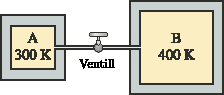
\includegraphics[width = 1.5in]{figures/ventill.pdf}
\end{wrapfigure}

\item \textit{(RK 18.73.)} Tvö ílát, $A$ og $B$ innihalda sama kjörgas. Rúmmálið í íláti $B$ er fjórum sinnum meira heldur en rúmmálið í $A$. Ílátin eru tengd saman með litlu röri (með hverfandi rúmmáli). Á rörinu er ventill sem hægt er að opna eða loka fyrir flæði á milli tankanna. Tanki $A$ er haldið við fast hitastig $\SI{300}{K}$ og tanki $B$ er haldið við fast hitastig $\SI{400}{K}$. Þrýstingurinn í tanki $A$ er til að byrja með $\SI{1}{atm}$ en þrýstingurinn í tanki $B$ er til að byrja með $\SI{5}{atm}$. Síðan er opnað fyrir ventilinn og gasið flæðir á milli tankanna þar til að þeir eru við sama þrýsting. Hver er sá þrýstingur?

\end{minipage}
\end{comment}

\end{enumerate}

\subsection*{Svör}

\begin{enumerate*}[label = \vspace{0.15cm} \textbf{(\arabic*)}]
\setcounter{enumi}{7}
  \item $P = \SI{18.8}{atm}$.
  \item $V = \SI{49.7}{L}$.
  \item $n = \SI{1.56}{mól}$, $N = \SI{9.4e23}{sameindir}$, $V = \SI{12,5}{L}$, $P = \SI{3.00}{atm}$, $v = \SI{478}{m/s}$.
  \item $h = \SI{23}{cm}$.
  \item $\Delta V = \SI{500}{mL}$, $W = \SI{86}{J}$.
  \item $r_2 = \SI{17}{cm}$.
\end{enumerate*}

\newpage

\subsection*{Fyrsta lögmál varmafræðinnar og varmaferli}

\begin{tcolorbox}
Fyrsta lögmál varmafræðinnar segir að fyrir kjörgas gildir að: $C_V n \Delta T = \Delta E = Q - W$, þar sem $Q$ er varmaorkan sem flyst inn í kerfið, $W$ er vinnan sem að kerfið vinnur og $\Delta E$ er heildarorkubreyting kerfisins. Hér er $C_V = \frac{f}{2}R$, þar sem $f$ táknar frelsisgráður sameindanna í gasinu og $R = \SI{8.315}{J/mól.K}$ er gasfastinn. Fjögur mikilvægustu varmaferlin og PV-línurit þeirra eru:
\begin{figure}[H]
    \centering
    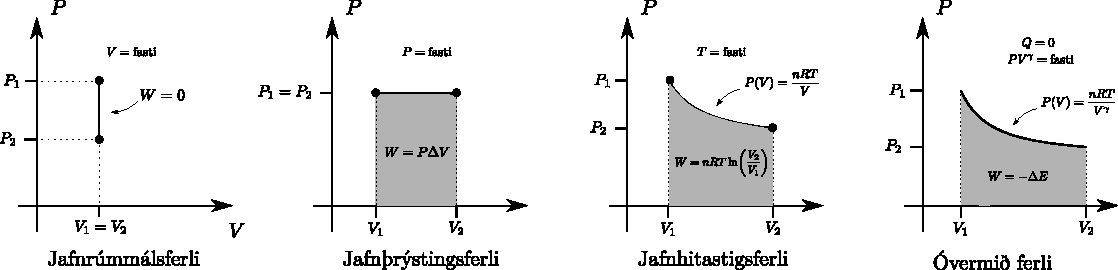
\includegraphics[width = \textwidth]{figures/varmaferlin.pdf}
\end{figure}
\end{tcolorbox}

\begin{enumerate}[label = \textbf{Dæmi \thechapter.\arabic*.}]

\setcounter{enumi}{13}


\begin{minipage}{\linewidth}

\begin{wrapfigure}{r}{1.5in}
\hspace{0.5cm}
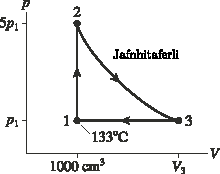
\includegraphics[width = 1.5in]{figures/pV-dia.pdf}
\begin{comment}
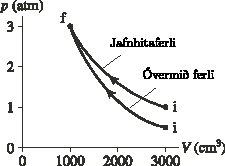
\includegraphics[width = 1.5in]{figures/adia-pv.pdf}
\end{comment}
\end{wrapfigure}

\item \textit{(RK 19.11.)} Við það að $\SI{500}{J}$ af vinnu var unninn á kjörgasi þá minnkaði heildarorka kerfisins um $\SI{200}{J}$. Hversu mikil varmaorka bættist inn í kerfið?

\item \textit{(RK 19.10.)} Kjörgasi er þjappað saman frá $\SI{600}{cm^3}$ niður í \SI{200}{cm^3} við fastann þrýsting \SI{400}{kPa}. Á sama tíma tapar gasið $\SI{100}{J}$ af varmaorku. Hver er heildarorkubreyting gassins í þessu ferli?

\item \textit{(RK. 19.62.)} Á PV-línuritinu hér til hægri má sjá varmahringrás sem \SI{0.03}{mól} af helíni fylgja. \begin{enumerate*}[label =\textbf{(\alph*)}]
    \item Ákvarðið þrýstinginn, hitastigið og rúmmálið í 1, 2 og 3.
    \item Hversu mikla vinnu vinnur gasið í hverjum hluta hringrásarinnar?
    \item Hversu mikilli varmaorku var bætt inn í kerfið í hverjum lið hringrásarinnar?
\end{enumerate*}

\begin{comment}
\item \textit{RK. 19.58.} Skoðum tvö mismunandi varmaferli sem að \SI{0.10}{mól} af niturgasi geta fylgt (hér til hægri). Annars vegar jafnhitaferli og hinsvegar óvermið ferli. Hversu mikil er \begin{enumerate*}[label = \textbf{(\alph*)}]
    \item varma-
    \item vinnu-
    \item heildarorku-
\end{enumerate*}breyting kerfisins í hvoru ferli um sig?
\end{comment}

\end{minipage}

\vspace{-0.25cm}

\item \textit{(RK 21.35.)} Á myndinni hér fyrir neðan má skrefin sem einföld varmavél tekur í einni hringrás. Massarnir ofan á bullunni eru þannig að í skrefum 3 og 6 þá er bullan í kraftajafnvægi. \begin{enumerate*}[label = \textbf{(\alph*)}]
    \item Teiknið PV-línurit fyrir þessa varmavél.
    \item Hversu mikla vinnu vinnur varmavélin í hverri hringrás?
    \item Varmanýttni er skilgreind sem $\eta := \frac{W_{\text{út}}}{Q_{\text{inn}}}$ þar sem $W_{\text{út}}$ er heildarvinnan sem gasið vinnur í einni hringrás og $Q_{\text{inn}}$ er (jákvæða) varmaorkan sem bætt var inn í kerfið í sömu hringrás. Hver er varmanýttni varmavélarinnar?
\end{enumerate*}

\vspace{-0.3cm}
\begin{figure}[H]
    \centering
    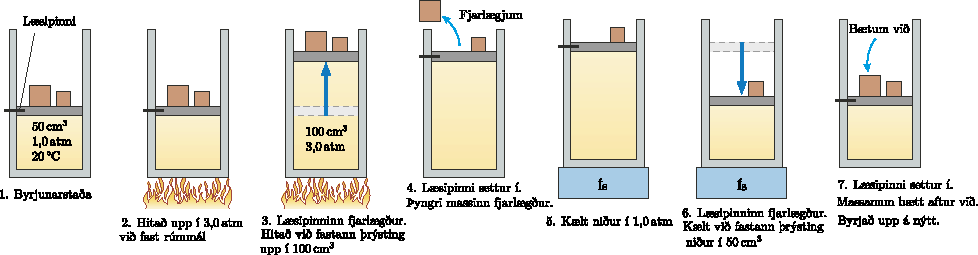
\includegraphics[width = \textwidth]{figures/varmavel.pdf}
\end{figure}

\end{enumerate}

\subsection*{Svör}

\begin{enumerate*}[label = \vspace{0.15cm} \textbf{(\arabic*)}]
\setcounter{enumi}{13}
  \item $Q= \SI{-700}{J}$
  \item $\Delta E = \SI{60}{J}$.
  \item $P_1 = P_3 = \SI{1.0}{atm}$, $P_2 = \SI{5.0}{atm}$, $T_2 = T_3 = \SI{1757}{\degree C}$, $V_3 = \SI{5000}{cm^3}$, $W_{12} = \SI{0}{J}$, $W_{23} = \SI{815}{J}$, $W_{31} = \SI{-405}{J}$, $Q_{12} = \SI{608}{J}$, $Q_{23} = \SI{815}{J}$, $Q_{31} = \SI{-1013}{J}$.
  \item $W_{12} = \SI{0}{J}$, $W_{23} = \SI{15.2}{J}$, $W_{34} = \SI{0}{J}$, $W_{41} = \SI{-5.1}{J}$, $W_{\text{heild}} = \SI{10.1}{J}$, $n = \SI{2.1}{mmól}$, $Q_{12} = \SI{15.3}{J}$, $Q_{23} = \SI{38.2}{J}$, $Q_{34} = \SI{-30.7}{J}$, $Q_{41} = \SI{-12.8}{J}$, $\eta = \SI{0.19}{}$.
\end{enumerate*}



%%%%%%%%%%%%%%%%%%%%%%%%%%%%%%%%
%      END OF CHAPTER TEXT 
%%%%%%%%%%%%%%%%%%%%%%%%%%%%%%%%
\ifdefined \wholebook \else
 \printindex
\end{document}
\fi